%-------------------------------------------------------------------------------------------------------
%-------------------------------------------------------------------------------------------------------
%-------------------------------------------------------------------------------------------------------
\subsection{Introducci\'on a la secci\'on}
Cada apartado es una simulaci\'on de la futura aplicaci\'on del algoritmo. Cada una consta de una escena propia mostrada como en la figura \ref{fig:VREP_scene_example}. El resultado se visualiza por consola en el formato que muestra la figura \ref{fig:Ground_Tracking_VREP_Console}. \\

\begin{figure}[ht]
	\centering
	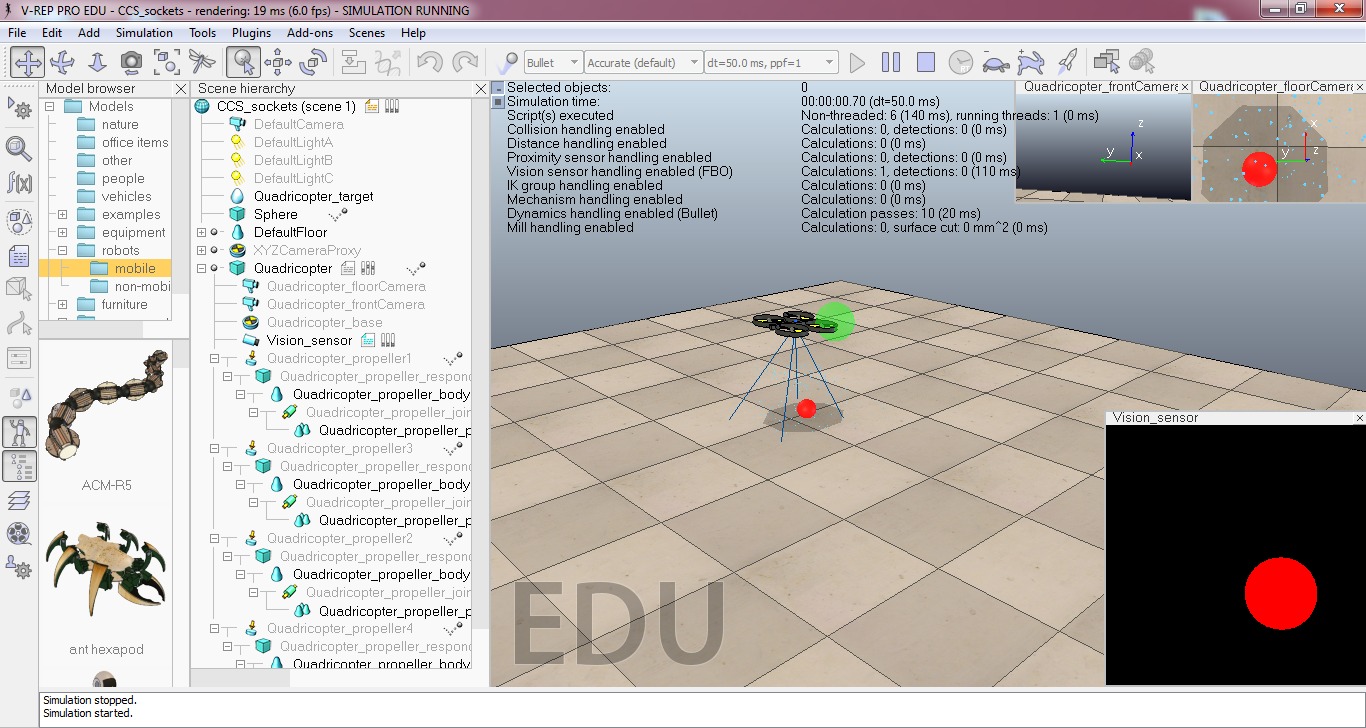
\includegraphics[width=0.8\textwidth,natwidth=1366,natheight=728]{../Images/c3/ground_tracking_scene.png}
	\caption{Ground Tracking Scene}
	\label{fig:VREP_scene_example}
\end{figure}

\begin{figure}[ht]
	\centering
	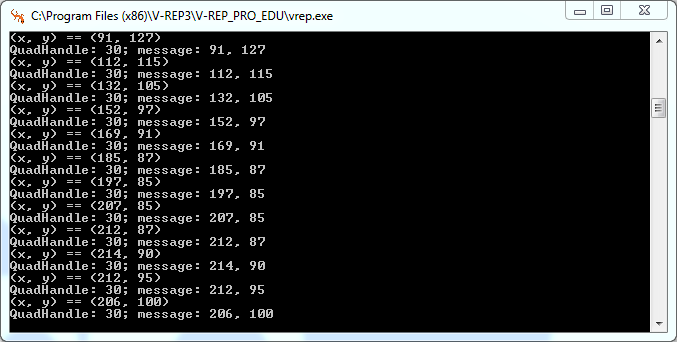
\includegraphics[width=0.8\textwidth,natwidth=677,natheight=342]{../Images/c3/ground_tracking_vrep_console.png}
	\caption{Ground Tracking V-REP Console}
	\label{fig:Ground_Tracking_VREP_Console}
\end{figure}

La estación en tierra se simula con una aplicaci\'on en el mismo ordenador que ejecuta la simualaci\'on tal que los resultados se muestran tambi\'en por consola del siguiente modo: \ref{fig:Ground_Tracking_Server_Console}.

\begin{figure}[ht]
	\centering
	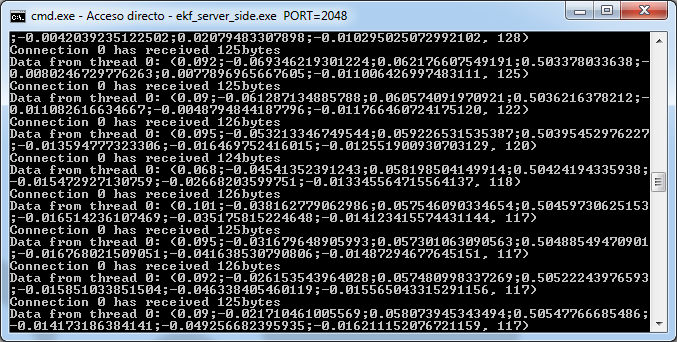
\includegraphics[width=0.8\textwidth,natwidth=677,natheight=342]{../Images/c3/ground_tracking_server_console.png}
	\caption{Ground Tracking Server Console}
	\label{fig:Ground_Tracking_Server_Console}
\end{figure}

Ambos procesos (Quadrotor y estaci\'on de tierra) generan unos ficheros de LOG que se usar\'an para analizar los resultados.

%-------------------------------------------------------------------------------------------------------
%-------------------------------------------------------------------------------------------------------
%-------------------------------------------------------------------------------------------------------
\subsection{Simulaci\'on 1 - Seguimiento de objeto de tierra con c\'amara vertical}
\subsubsection{Preparaci\'on}
La escena consta de un dron y un objetivo (Figure: \ref{fig:VREP_scene_example}). La c\'amara apunta hacia el suelo y el quadrotor sigue al objetivo con los datos extraídos del algoritmo de visi\'on (Figure: \ref{fig:ground_tracking_scene_vertical}).

\begin{figure}[ht]
	\centering
	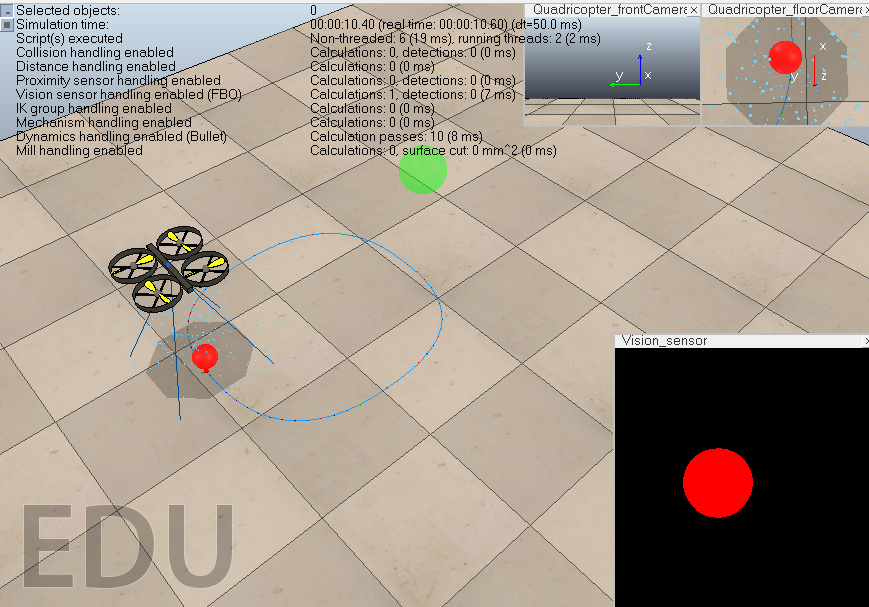
\includegraphics[width=0.65\linewidth]{../Images/c3/ground_tracking_scene_vertical}
	\caption{Ground tracking - Oblique Camera}
	\label{fig:ground_tracking_scene_vertical}
\end{figure}

\subsubsection{Test y resultados}

	En este test el error m\'aximo es de 1 cm al inicio del algoritmo, posteriormente es $\sim$ 0. La primera figura muestra las coordenadas reales y calculadas del objetivo (\ref{fig:sim1_traj_ori} and \ref{fig:sim1_traj_track}) y la segunda figura la trayectoria en tres dimensiones \ref{fig:sim1_traj_both_3d}.
	
\begin{figure}[htp]
	\centering
	\begin{subfigure}{0.45\linewidth}
		\centering
		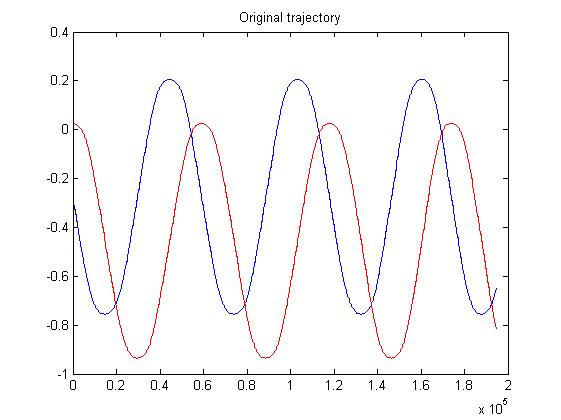
\includegraphics[width=\linewidth]{../Images/c3/sim1_traj_ori}
		\caption{Seguimiento terrestre - Trayectoria Original}
		\label{fig:sim1_traj_ori}
	\end{subfigure}
	~
	\begin{subfigure}{0.45\linewidth}
		\centering
		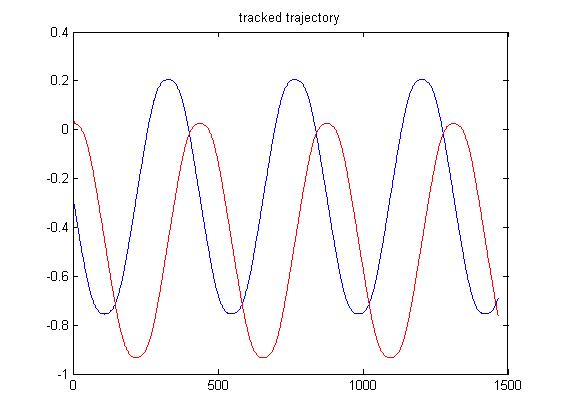
\includegraphics[width=\linewidth]{../Images/c3/sim1_traj_track}
		\caption{Seguimiento terrestre - Trayectoria calculada}
		\label{fig:sim1_traj_track}
	\end{subfigure}

\end{figure}


\begin{figure}[ht]
\centering
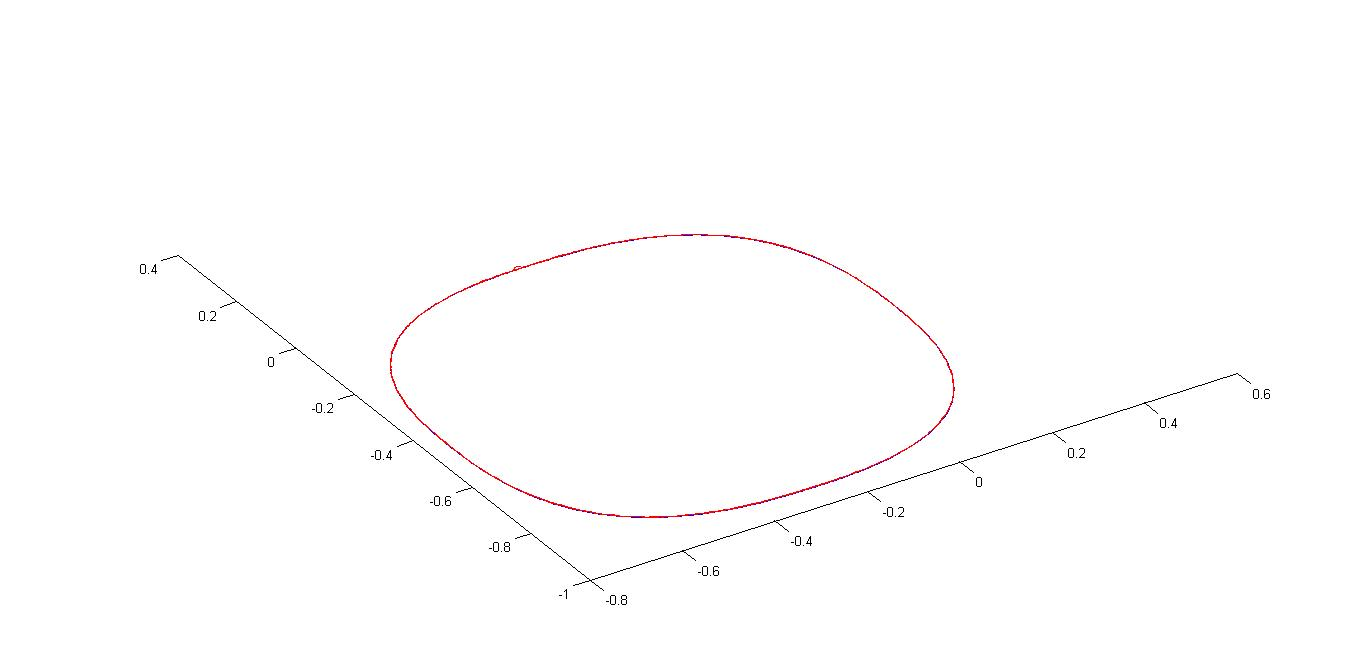
\includegraphics[width=0.7\linewidth]{../Images/c3/sim1_traj_both_3d}
\caption{Seguimiento terrestre - Trayectoria tridimensional}
\label{fig:sim1_traj_both_3d}
\end{figure}




%-------------------------------------------------------------------------------------------------------
%-------------------------------------------------------------------------------------------------------
%-------------------------------------------------------------------------------------------------------
\subsection{Simulaci\'on 2 - Seguimiento terrestre con c\'amara oblicua}
\subsubsection{Preparaci\'on}
Esta escena es pr\'acticamente la anterior, salvo que la c\'amara ya no se encuentra vertical sino oblicua (A 45 grados respecto al eje vertical) \ref{fig:ground_tracking_scene_oblique}). Para esta prueba adem\'as se aument\'o la velocidad del objetivo:

\begin{figure}[hp]
	\centering
	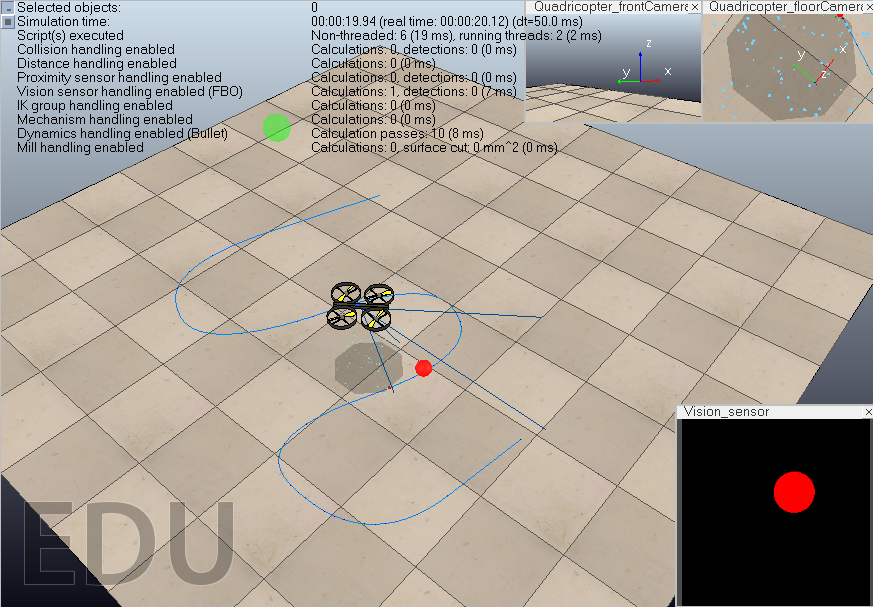
\includegraphics[width=0.65\linewidth]{../Images/c3/ground_tracking_scene_oblique}
	\caption{Seguimiento terrestre - C\'amara oblicua}
	\label{fig:ground_tracking_scene_oblique}
\end{figure}

\subsubsection{Test y resultados}
\label{lab:sim2_test_results}
El error inicial m\'aximo es de $\sim$ 2 cm debido a la velocidad inicial del objetivo respecto a la din\'amica del quadrotor. En adelante el error es $\sim$ 0. La primera figura muestra las trayectorias original y calculadas (\ref{fig:sim2_traj_ori} y \ref{fig:sim2_traj_track}), y finalmente se muestra la reconstrucci\'on 3D de la trayectoria. \ref{fig:sim2_traj_both_3d}.

\begin{figure}[htp]
	\centering
	\begin{subfigure}[htp]{0.48\linewidth}
		\centering
		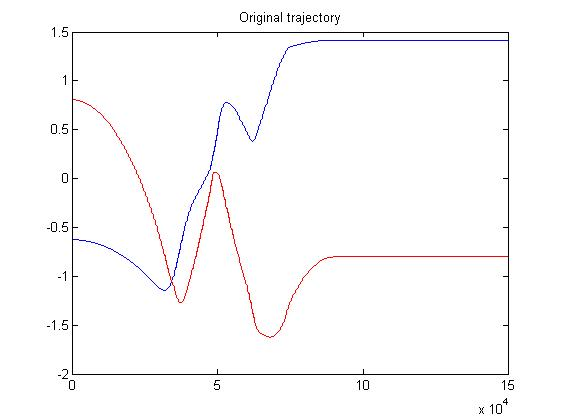
\includegraphics[width=\linewidth]{../Images/c3/sim2_traj_ori}
		\caption{Seguimiento terrestre - Trayectoria original}
		\label{fig:sim2_traj_ori}
	\end{subfigure}
	~
	\begin{subfigure}[htp]{0.48\linewidth}
		\centering
		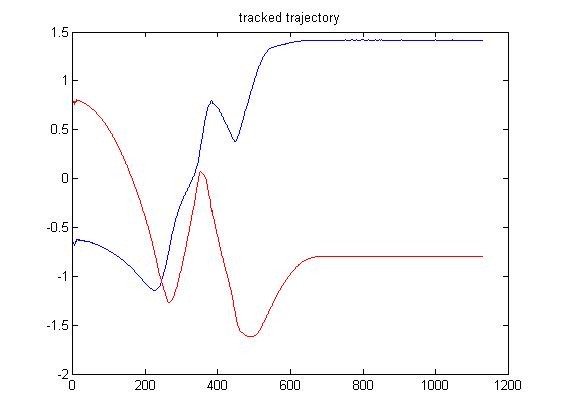
\includegraphics[width=\linewidth]{../Images/c3/sim2_traj_track}
		\caption{Seguimiento terrestre - Trayectoria calculada}
		\label{fig:sim2_traj_track}
	\end{subfigure}

\end{figure}


\begin{figure}[h]
\centering
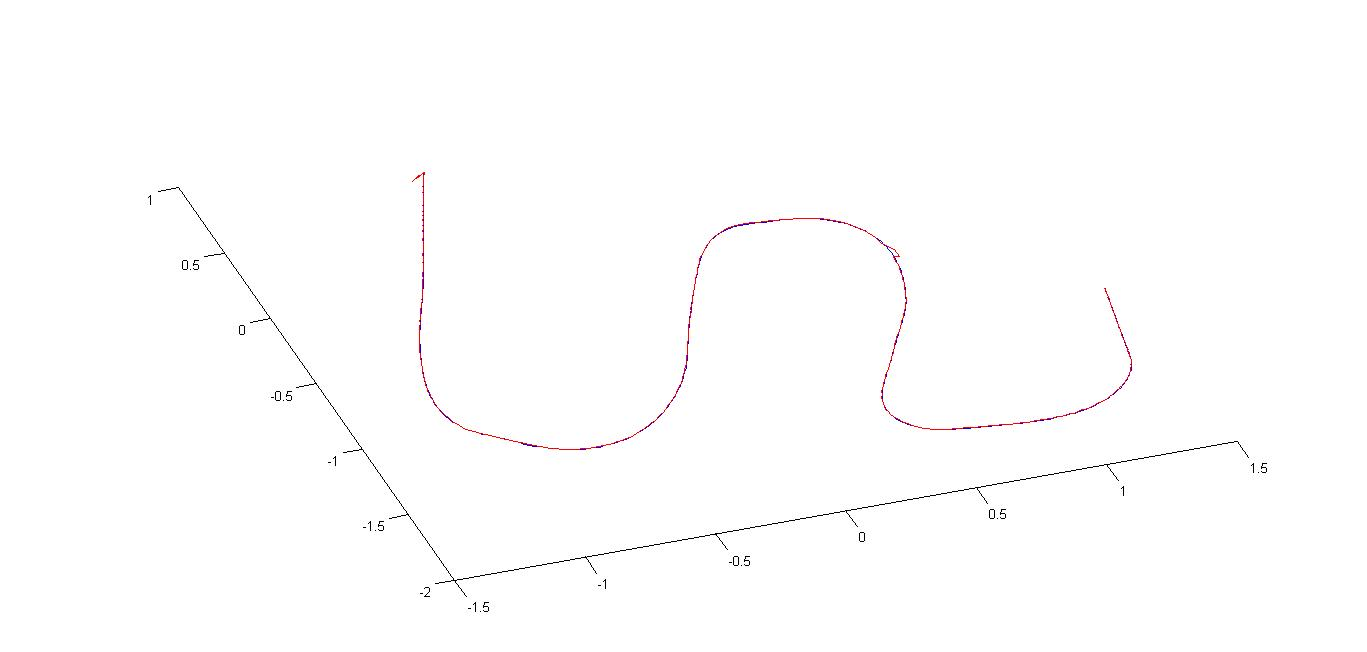
\includegraphics[width=0.9\linewidth]{../Images/c3/sim2_traj_both_3d}
\caption{Seguimiento terrestre - Trayectoria tridimensional}
\label{fig:sim2_traj_both_3d}
\end{figure}




%-------------------------------------------------------------------------------------------------------
%-------------------------------------------------------------------------------------------------------
%-------------------------------------------------------------------------------------------------------
\subsection{Simulaci\'on 3 - Seguimiento Est\'ereo}
\subsubsection{Preparaci\'on}
Esta simulaci\'on dos quadrotors y un objetivo como se ve en la figura \ref{fig:sim3_set_up}.

\begin{figure}[htp]
	\centering
	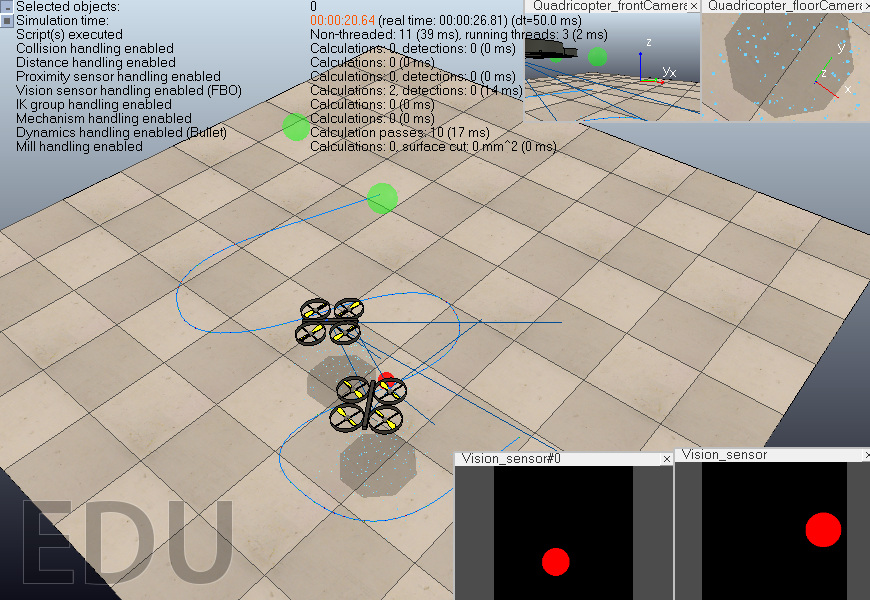
\includegraphics[width=0.4\linewidth]{../Images/c3/sim3_set_up}
	\caption{Seguimiento Est\'ereo}
	\label{fig:sim3_set_up}
\end{figure}


%\begin{figure}[h]
%	\centering
%	\begin{subfigure}[b]{0.4\linewidth}
%	\centering
%		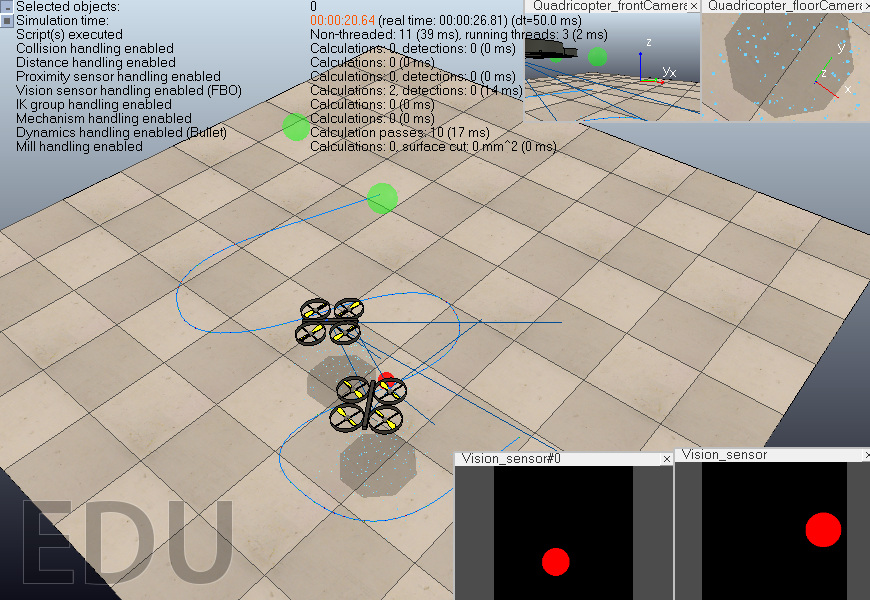
\includegraphics[width=\linewidth]{../Images/c3/sim3_set_up}
%		\caption{Stereo tracking - Set up}
%		\label{fig:sim3_set_up}
%	\end{subfigure}
%	~
%	\begin{subfigure}[b]{0.4\linewidth}
%		\centering
%		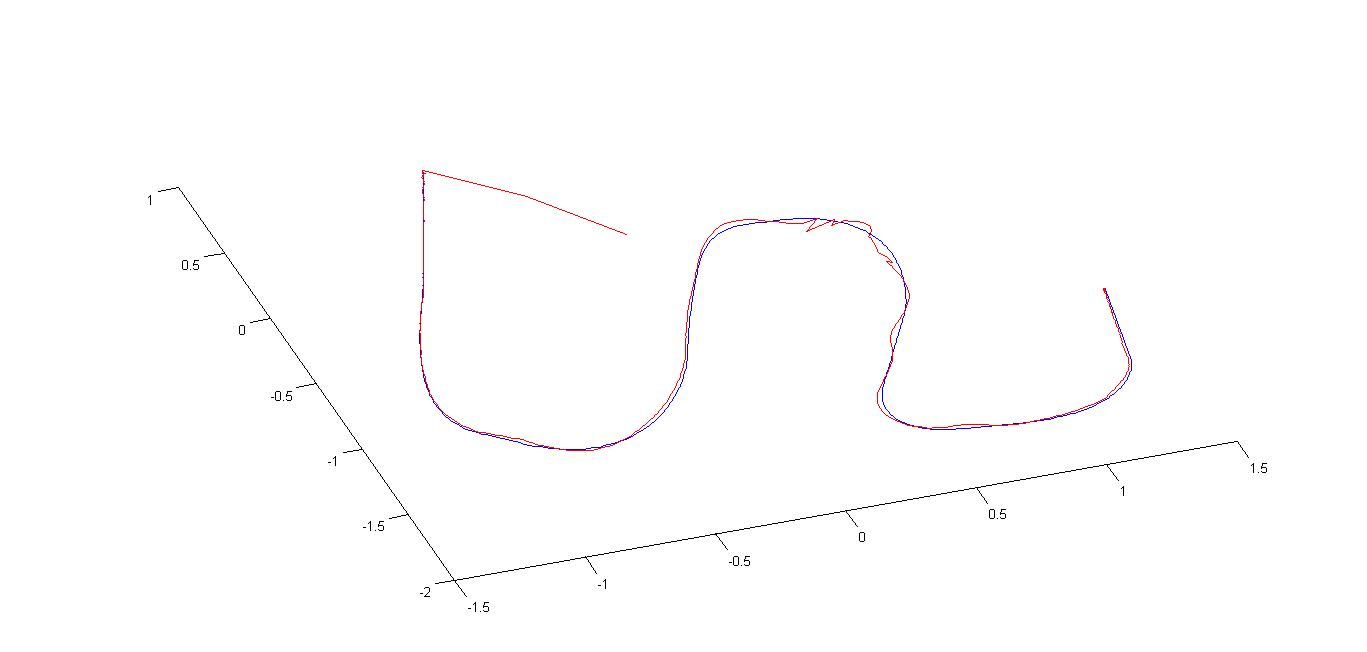
\includegraphics[width=\linewidth]{../Images/c3/sim3_traj_both_3d}
%		\caption{Stereo tracking - 3D trajectory}
%		\label{fig:sim3_traj_both_3d}
%	\end{subfigure}
%\end{figure}

\subsubsection{Test and results}

	En esta simulaci\'on el error m\'aximo es $\sim$ 3 cm. y el m\'inimo $\sim$ 1 cm. El error m\'aximo se encuentra al final de la curva debido al aumento de velocidad del objetivo en esa parte \ref{fig:sim3_traj_both_3d}.
	

\begin{figure}[hp]
	\centering
	\begin{subfigure}[hp]{0.4\linewidth}
		\centering
		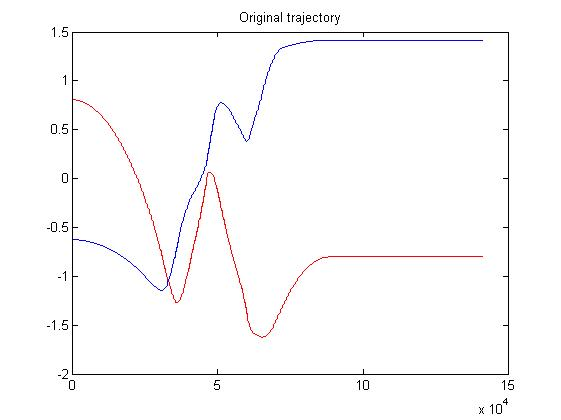
\includegraphics[width=\linewidth]{../Images/c3/sim3_traj_ori}
		\caption{Seguimiento Est\'ereo - Trayectoria Original}
		\label{fig:sim3_traj_ori}
	\end{subfigure}
	~
	\begin{subfigure}[hp]{0.4\linewidth}
		\centering
		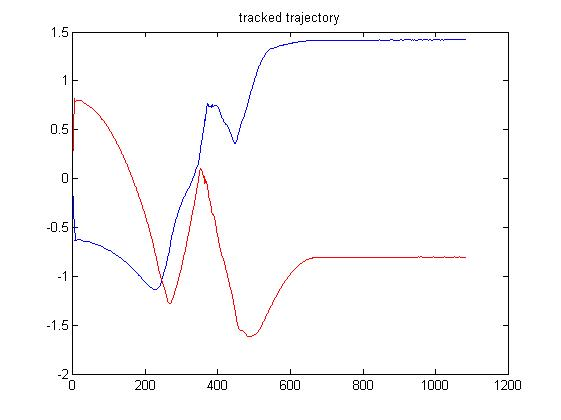
\includegraphics[width=\linewidth]{../Images/c3/sim3_traj_track}
		\caption{Seguimiento Est\'ereo - Trayectoria Calculada}
		\label{fig:sim3_traj_track}
	\end{subfigure}
\end{figure}

\begin{figure}[htp]
		\centering
		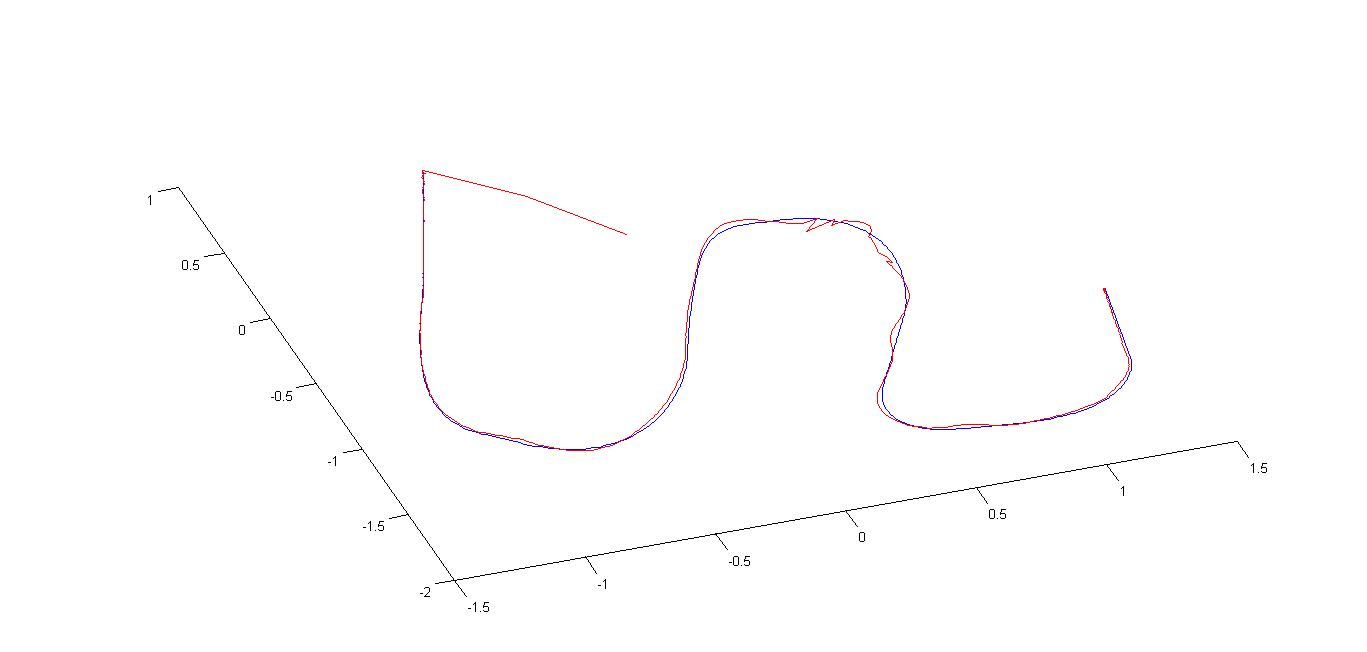
\includegraphics[width=0.4\linewidth]{../Images/c3/sim3_traj_both_3d}
		\caption{Stereo tracking - 3D trajectory}
		\label{fig:sim3_traj_both_3d}
\end{figure}

%-------------------------------------------------------------------------------------------------------
%-------------------------------------------------------------------------------------------------------
%-------------------------------------------------------------------------------------------------------
\subsection{Simulaci\'n 4 - Seguimiento en tierra de m\'ultiples objetivos}
\subsubsection{Preparaci\'on}
 Este experimento consta de un solo quadrotor y dos obetivos \ref{fig:sim4_set_up}.
 
\begin{figure}[htp]
	\centering
	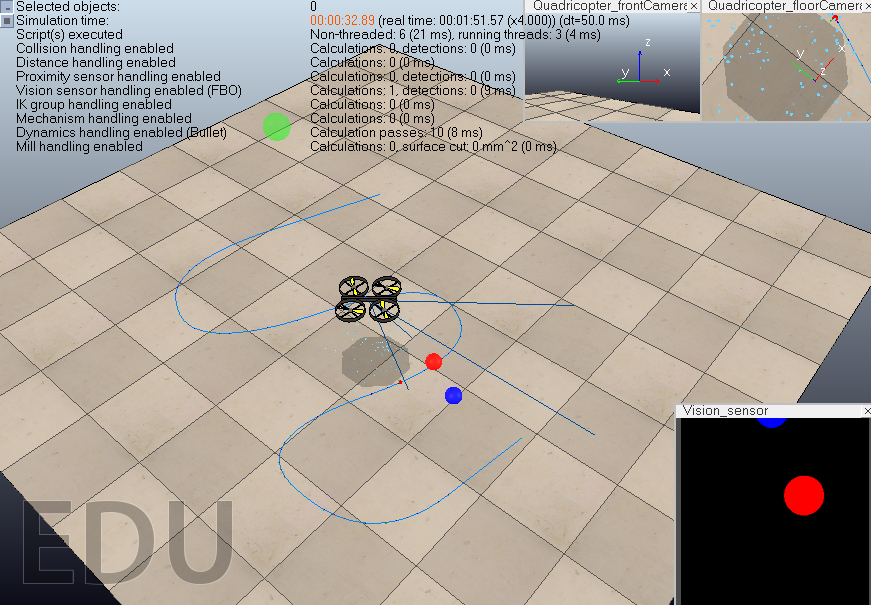
\includegraphics[width=0.4\linewidth]{../Images/c3/sim4_set_up}
	\caption{Objetivos M\'ultiples objetivos}
	\label{fig:sim4_set_up}
\end{figure}

\subsubsection{Test y resultados}

	Como en los apartados anteriores se muestran tres figuras correspondientes a las coordenadas XY original y calculada y la trayectoria 3D (\ref{fig:sim4_redtarget}, \ref{fig:sim4_bluetarget} y \ref{fig:sim4_3dtraj}). \\
	
	\begin{figure}[hp]
		\centering
		\begin{subfigure}[hp]{0.45\linewidth}
			\centering
			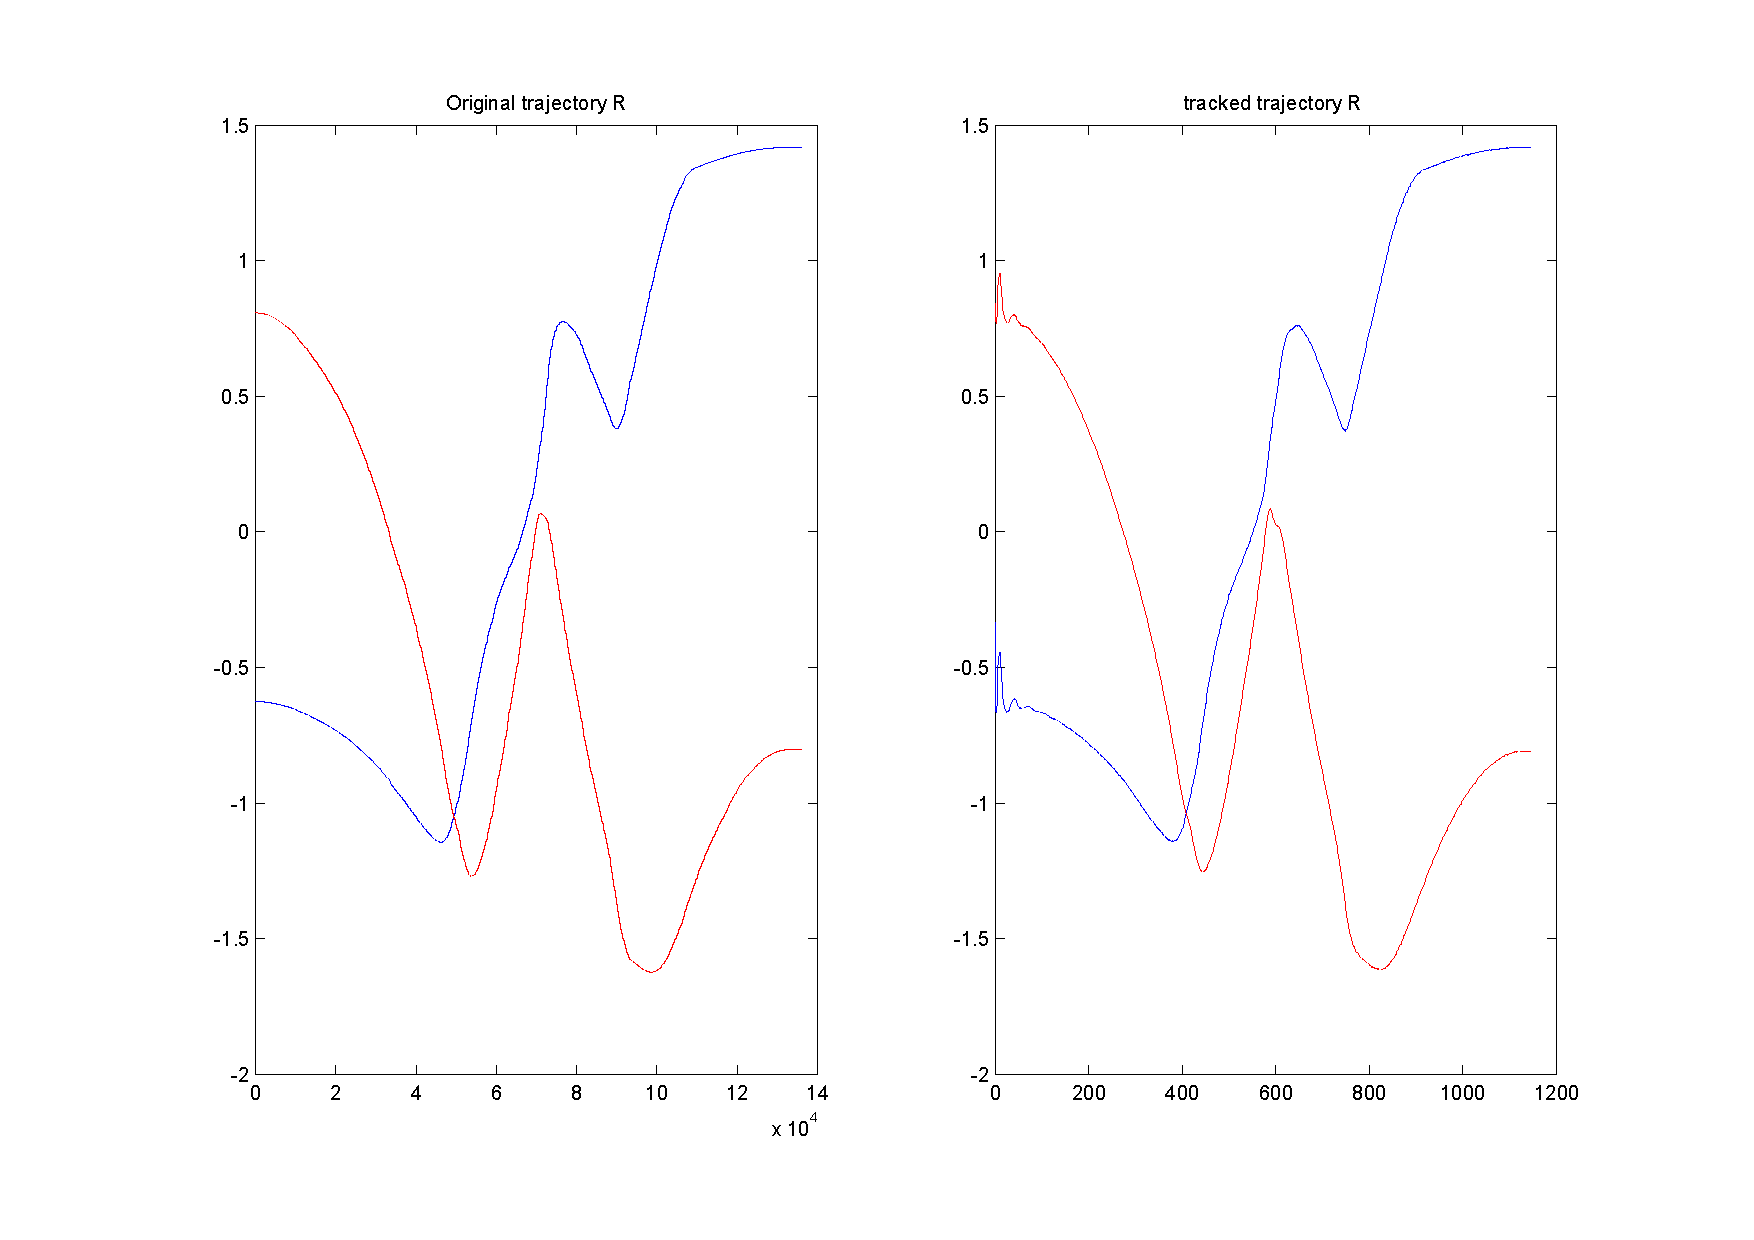
\includegraphics[width=\linewidth]{../Images/c3/sim4_redtarget}
			\caption{Multiple Targets - Red target}
			\label{fig:sim4_redtarget}	
		\end{subfigure}
		~
		\begin{subfigure}[hp]{0.45\linewidth}
			\centering
			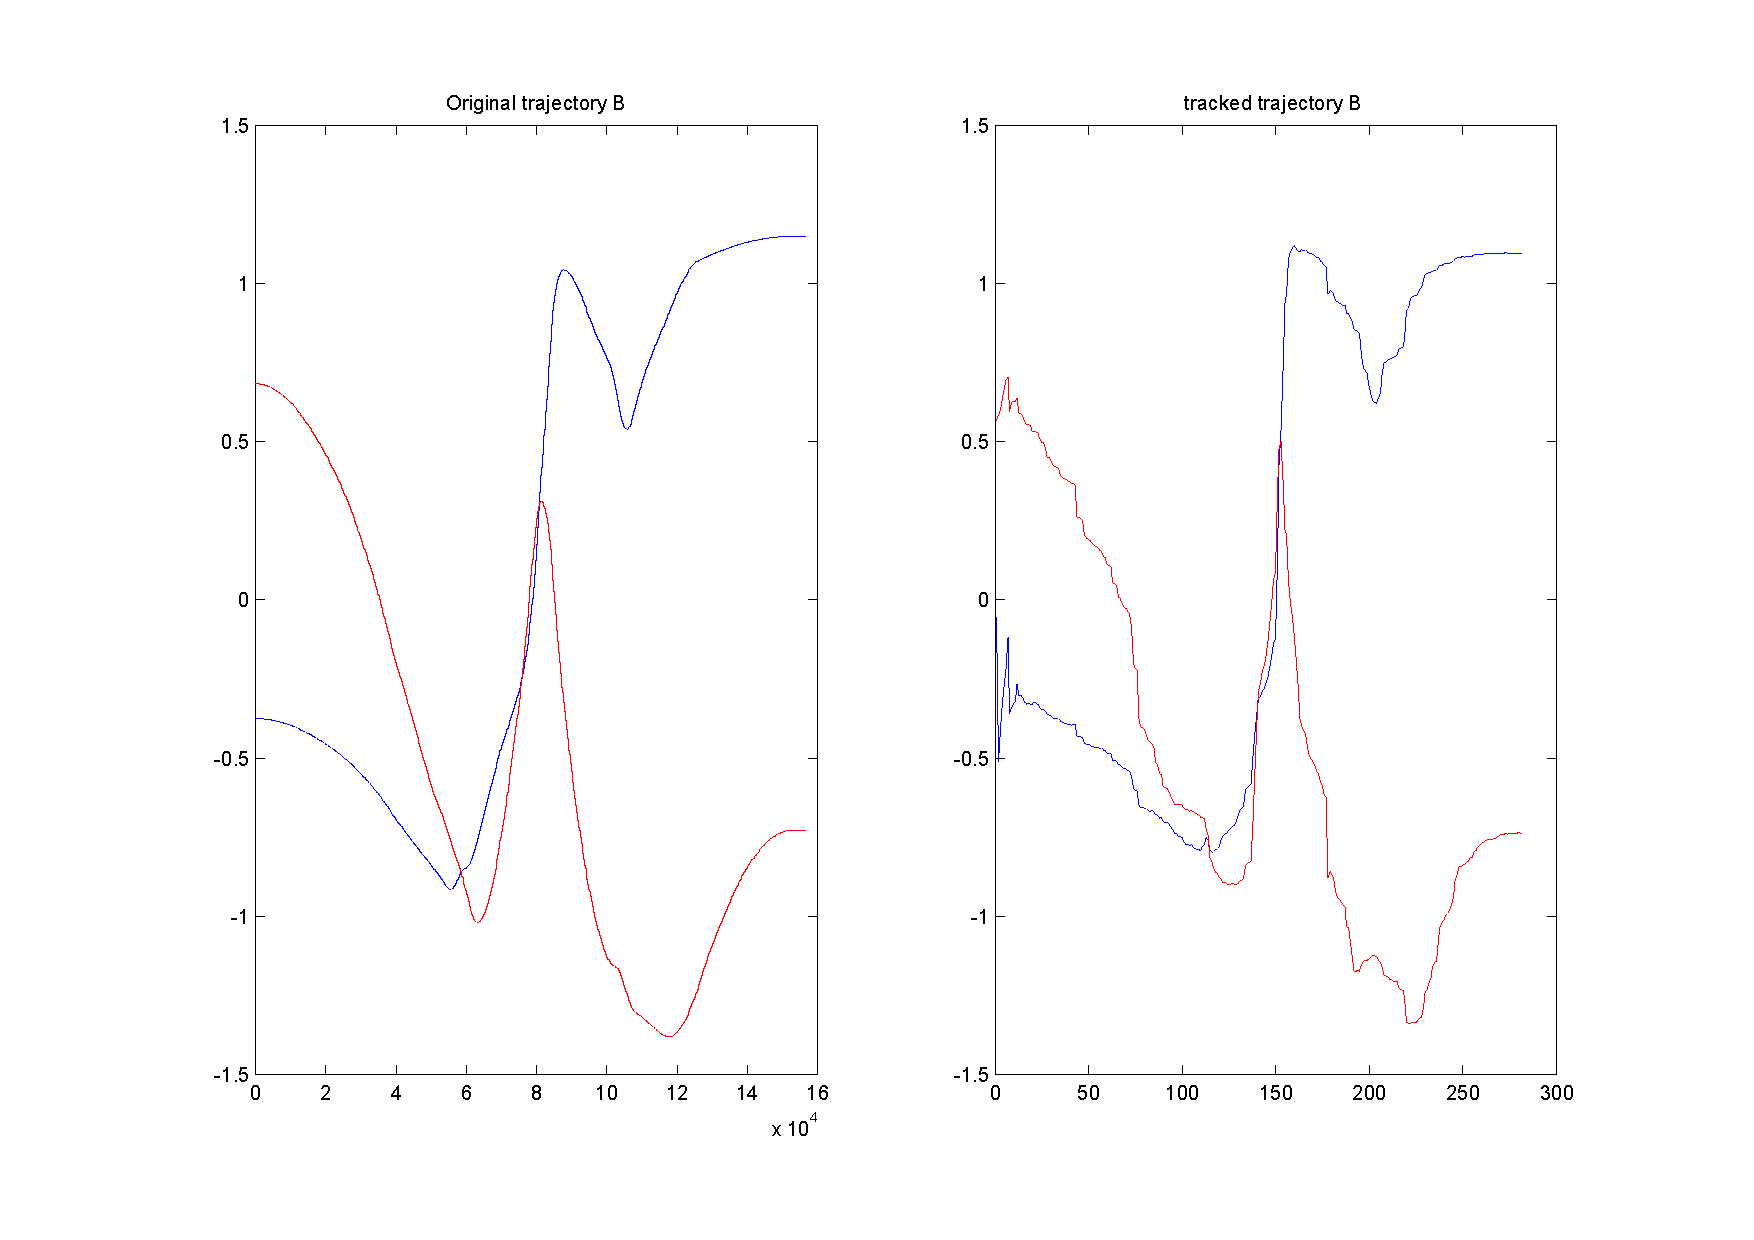
\includegraphics[width=\linewidth]{../Images/c3/sim4_bluetarget}
			\caption{Multiple Targets - Blue target}
			\label{fig:sim4_bluetarget}
		\end{subfigure}
	\end{figure}
	
	Los resultados esta simulaci\'on son buenos igual que en los apartados anteriores \ref{fig:sim2_traj_both_3d}. El resultado del seguimiento del objeto azul puede parecer erroneo inicialmente, sin embargo es un resultado totalmente coherente ya que este nunca se ve completamente por lo que nunca se obtiene el centro real del mismo \ref{fig:sim4_centroid_objs} y de ah\'i el error en posici\'on. El error m\'aximo en el azul es $\sim$ 15 cm y el medio es $\sim$ 6 cm.



\begin{figure}[hp]
	\centering
	\begin{subfigure}{0.45\linewidth}
		\centering
		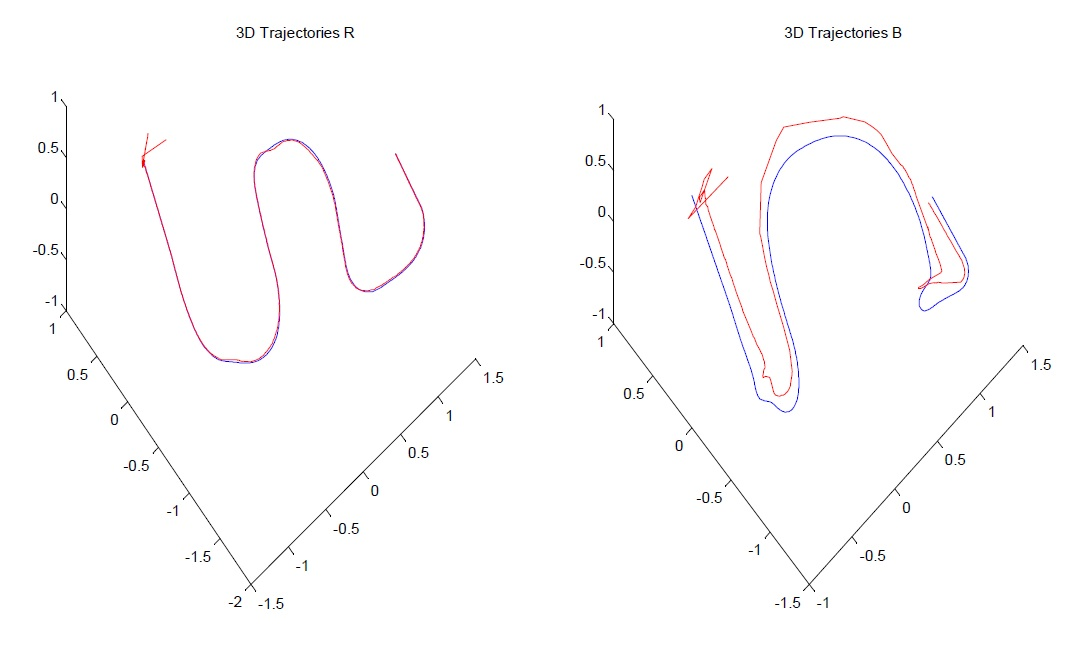
\includegraphics[width=\linewidth]{../Images/c3/sim4_3dtraj}
		\caption{M\'ultiples objetivos - Trayectoria 3D}
		\label{fig:sim4_3dtraj}
	\end{subfigure}
	~
	\begin{subfigure}{0.2\linewidth}
		\centering
		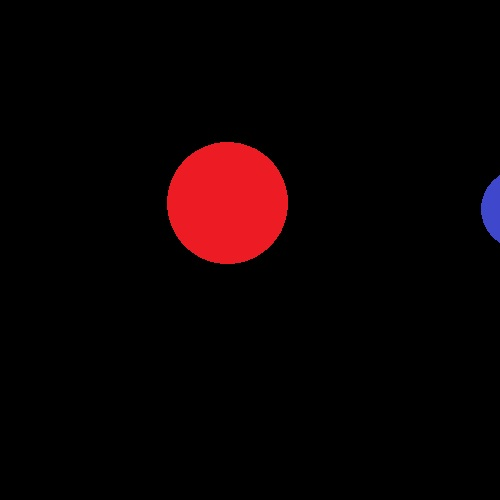
\includegraphics[width=\linewidth]{../Images/c3/sims_two_object_centroid_out}
		\caption{M\'ultiples objetivos - Centroides}
		\label{fig:sim4_centroid_objs}
	\end{subfigure}
\end{figure}